% Default mode is landscape, which is what we want, however dvips and
% a0poster do not quite do the right thing, so we end up with text in
% landscape style (wide and short) down a portrait page (narrow and
% long). Printing this onto the a0 printer chops the right hand edge.
% However, 'psnup' can save the day, reorienting the text so that the
% poster prints lengthways down an a0 portrait bounding box.
%
% 'psnup -w85cm -h119cm -f poster_from_dvips.ps poster_in_landscape.ps'

\documentclass[a0]{a0poster}
% You might find the 'draft' option to a0 poster useful if you have
% lots of graphics, because they can take some time to process and
% display. (\documentclass[a0,draft]{a0poster})

\pagestyle{empty}
\renewcommand{\d}{\mathrm{d}}
\newcommand{\sgn}[1]{\mathop{\mathrm{sgn}}#1}
\newcommand{\bu}{\mathbf{u}}
\newcommand{\bx}{\mathbf{x}}
\newcommand{\br}{\mathbf{r}}
\newcommand{\ds}{\mathrm{d}s}
\newcommand{\ie}{\textit{i.e.}}
\setcounter{secnumdepth}{0}
\newcommand{\comment}[1]{}

% The textpos package is necessary to position textblocks at arbitary 
% places on the page.
\usepackage[absolute]{textpos}

% Graphics to include graphics. Times is nice on posters, but you
% might want to switch it off and go for CMR fonts.
\usepackage[final]{graphics}
\usepackage{wrapfig,helvet}
\usepackage{amsmath}

% These colours are tried and tested for titles and headers. Don't
% over use color!
\usepackage{color}
\definecolor{DarkBlue}{rgb}{0.1,0.1,0.5}
\definecolor{Red}{rgb}{0.9,0.0,0.1}
\definecolor{headingcol}{rgb}{0.5,0.7,1}
%\definecolor{boxcol}{rgb}{0.3,0.8,0.1}

% see documentation for a0poster class for the size options here
\let\Textsize\normalsize
\def\Head#1{\noindent\hbox to \hsize{\hfil{\LARGE\color{DarkBlue}\sf #1}}\bigskip}
\def\LHead#1{\noindent{\LARGE\color{DarkBlue}\sf #1}\bigskip}
\def\Subhead#1{\noindent{\large\color{DarkBlue}\sf #1}\bigskip}
\def\Title#1{\noindent{\VeryHuge\color{Red}\bf\sf #1}}

\TPGrid[40mm,40mm]{23}{12}  % 3 cols of width 7 plus 2 gaps width 1

\parindent=0pt
\parskip=0.5\baselineskip

\makeatletter							%Needed to include code in main file
\renewcommand\@maketitle{%
\null									%Sets position marker
{
\color{headingcol}\sffamily\VERYHuge		%Set title font and colour
\@title \par}%
\vskip 0.6em%
{
\color{white}\sffamily\LARGE				%Set author font and colour
\lineskip .5em%
\begin{tabular}[t]{l}%
\@author
\end{tabular}\par}%
\vskip 1cm
\par
}
\makeatother

\title{Sample UCL-styled A0 scientific poster \LaTeX}

\author{Helen Wilson (with credit to Ed Long, CoMPLEX)\\ University College London}

\begin{document}
%----------------------------------------------------------------------%
%           Title bar: across all 21 columns                           %
%----------------------------------------------------------------------%
\begin{textblock}{23}(0,0)
\vspace*{-48mm}\hspace*{-42mm}%

\includegraphics{ucl_bar_black.eps}
\begin{minipage}{1191mm}		%Minipage for title contents
\vspace{-20cm}
\maketitle
\end{minipage}
\end{textblock}

%%%%%%%%%%%%%%%%%% Will need to shift all other content down a bit %%%%%

%----------------------------------------------------------------------%
%           First column.                                              %
%----------------------------------------------------------------------%
\begin{textblock}{7}(0,2.4)
\Head{Introductory segment}

\sf % Selects sans serif family: part of the UCL corporate image!
Lorem ipsum dolor sit amet, consectetuer adipiscing elit. Vestibulum justo. Praesent leo. Sed consectetuer. Aenean pretium, diam quis mattis porttitor, elit velit scelerisque sapien, sed convallis ipsum lectus non neque. Morbi in mi eu neque luctus scelerisque. Curabitur odio. Mauris a mi. Aenean iaculis erat vel sapien. Curabitur nulla velit, feugiat quis, imperdiet sit amet, vestibulum ac, diam. Suspendisse a metus. Pellentesque vulputate venenatis eros. In auctor, eros nec sodales faucibus, erat nisl facilisis nisl, ut rutrum nisl nunc eu est. Quisque eget ante at nunc varius ultrices.

\bigskip
\hrule
\end{textblock}

\begin{textblock}{7}(0,4.52)

\Head{First Piece of Content}

\sf 
It is worth fiddling around a bit with positioning of the text blocks to get the spacing even. I like a vertical gap of about 0.4 ``block units'' between the horizontal bar at the end of one block and the beginning of the next. There are contruction lines at the end of the \TeX\ file to help with this.

\begin{center}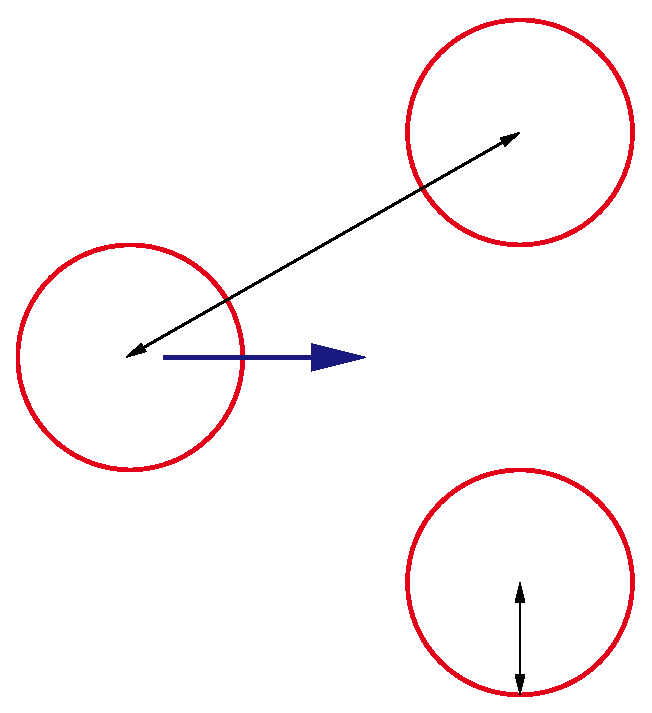
\includegraphics{fig1.eps}\end{center}
\begin{picture}(0,0)
\put(435,295){$aL$} 
\put(550,80){$a$}
\put(510,210){\textcolor{DarkBlue}{$F=6\pi\mu a$}}
\end{picture}

Figures (and labels using the \LaTeX\ picture environment) work as you would expect. 

\bigskip
\hrule
\end{textblock}

\begin{textblock}{7}(0,8.70)

\Head{Second Piece of Content}

\sf
Sed metus erat, bibendum ac, congue vitae, mattis et, dolor. Maecenas placerat mauris vel purus. Quisque molestie. Morbi eu mi in nibh venenatis aliquet. Pellentesque dapibus sem eget nibh. Donec sit amet felis. Cras lobortis blandit mauris. Cras non augue. Nullam lobortis risus in augue sodales sollicitudin. Proin vulputate gravida mauris. Sed dictum nunc id turpis. Mauris facilisis condimentum nisl. Aliquam tincidunt risus in tellus. Suspendisse dictum laoreet tellus. In hac habitasse platea dictumst. Proin suscipit, tellus ut molestie pulvinar, velit arcu lobortis neque, nec tempus neque sapien quis turpis. Aliquam accumsan. Ut eros mi, iaculis eu, tempor eu, placerat eget, nisi. Morbi nec justo eu sem fermentum accumsan. Nullam quis ipsum.

Vestibulum tincidunt, odio sed tincidunt lobortis, ante pede lacinia neque, a tempus magna dui in massa. Duis accumsan fermentum eros. Vivamus at mauris viverra odio porta venenatis. Nunc sed massa. Fusce hendrerit, lorem eu sollicitudin dapibus, nisi leo vestibulum ligula, in viverra lacus massa vel augue. Curabitur et nisi id dui dignissim blandit. Sed et nisi accumsan ipsum congue imperdiet. Suspendisse volutpat accumsan metus. Morbi est orci, sagittis in, dignissim id, interdum eu, libero. Maecenas hendrerit. Nulla sed magna. Cras tincidunt. Nulla sodales dictum lorem. Curabitur et neque. 

\bigskip
\hrule
\end{textblock}

%----------------------------------------------------------------------%
%           Second column.                                             %
%----------------------------------------------------------------------%
\begin{textblock}{7}(8,2.4)
\Head{Use of Colour}

\sf
With the {\tt color} package you can use as much colour as you like: but the \textcolor{Red}{Red} and \textcolor{DarkBlue}{DarkBlue} colours defined here are more useful than the obvious \textcolor{red}{red} and \textcolor{blue}{blue} versions, which tend to seem too bright when printed.

Use spacing as well as colour to highlight a key question or issue: 
\vspace*{1.15\baselineskip}
\begin{center}
\textcolor{Red}{Who will rid me of this turbulent priest?}
\end{center} 
\vspace*{1.15\baselineskip}
Praesent elementum malesuada mauris. Duis aliquet dolor ut nunc. Pellentesque euismod augue a odio. 

\bigskip
\hrule
\end{textblock}

\begin{textblock}{7}(8,5.25)

\Head{Equations and Tables}

\sf
Of course, the principal reason for choosing \LaTeX\ is its ability with equations:  
\[ 
   U_\mathrm{doublet} = \frac{mg}{2\pi\mu a}\left( \int_0^\infty \left\{ 1
       - \frac{2\sinh^2{s} - 2s^2}{\sinh{2s}+2s}\right\}\,\ds
   \right)^{-1} \approx \frac{1.55mg}{6\pi\mu a}, \] 
but it's equally easy to include tables: 
\begin{center} 
\begin{tabular}{cccccccccccr}
\hline
  && \multicolumn{2}{c}{$U_1$}  && \multicolumn{2}{c}{$U_2$} 
  && \multicolumn{2}{c}{$U_3$} & $U_3$ \\ 
$L$ &&    MR   &   SD   &&   MR   &   SD   &&   MR    &   SD & error \\ 
\hline
2.01 &&0.65528 &0.64739 &&0.63461 &0.62691 &&0.00498 &0.00451 & 9\%\\ 
2.10 &&0.73857 &0.73126 &&0.59718 &0.58784 &&0.03517 &0.02570 &27\%\\ 
2.50 &&0.87765 &0.87482 &&0.49545 &0.48829 &&0.07393 &0.05853 &21\%\\ 
3.00 &&0.93905 &0.93806 &&0.41694 &0.41356 &&0.07824 &0.06970 &11\%\\ 
4.00 &&0.97964 &0.97945 &&0.31859 &0.31774 &&0.06925 &0.06639 & 4\%\\ 
6.00 &&0.99581 &0.99579 &&0.21586 &0.21575 &&0.05078 &0.05019 & 1\%\\ 
\hline
\end{tabular} 
\end{center}
and, of course, images:
\begin{center}
\rotatebox{-90}{\scalebox{2.22}{\includegraphics{fig2.eps}}}
\end{center}

\bigskip
\hrule
\end{textblock}

%----------------------------------------------------------------------%
%           Third column.                                              %
%----------------------------------------------------------------------%
\begin{textblock}{7}(16,2.4)

\Head{Sectioning}

\Subhead{First Subsection}

\sf
Aenean feugiat, mauris vitae accumsan venenatis, tortor nunc facilisis velit, vel aliquam felis dui non ante. Aenean commodo, sem vel malesuada placerat, erat lacus lacinia magna, quis euismod quam nulla vitae turpis. Vivamus sapien. Vestibulum ante ipsum primis in faucibus orci luctus et ultrices posuere cubilia Curae; Nunc a dolor. Sed diam leo, fringilla non, fermentum non, ultricies tempor, dolor. Mauris vehicula, urna ac bibendum scelerisque, enim nisl vehicula libero, id blandit enim lacus et neque. Nunc posuere elit at erat. Integer commodo, eros dapibus blandit facilisis, dolor ipsum dictum dui, sit amet iaculis enim elit sed magna. Nunc libero nunc, malesuada sit amet, tincidunt at, pharetra ut, arcu.

\bigskip

\Subhead{Second Subsection}

Integer ante. Mauris tincidunt adipiscing mi. Donec sollicitudin, lacus quis pellentesque placerat, quam elit pharetra lacus, sit amet placerat nisi quam in lorem. Etiam id nulla a est vestibulum tempus. Nam et nisl non arcu venenatis semper. Duis sed libero. Cras lectus. In semper urna in leo. Sed mattis lacinia arcu. Phasellus ut metus. Phasellus mi dolor, condimentum ut, ornare nec, tempus ac, mi. Integer ante sem, vestibulum in, gravida vel, condimentum non, ipsum.

\bigskip
\hrule
\end{textblock}


\begin{textblock}{7}(16,6.85)

\Head{Discussion and Conclusions}

\sf
Etiam sit amet nisi. Lorem ipsum dolor sit amet, consectetuer adipiscing elit. Phasellus pharetra lacus. Aliquam erat volutpat. Donec leo. Mauris dapibus, magna sed hendrerit volutpat, massa magna euismod metus, vel gravida purus odio eget neque. Proin nibh turpis, commodo at, viverra sed, auctor vel, turpis. Mauris massa lacus, malesuada at, consectetuer at, condimentum non, nibh. Sed laoreet, lorem non tristique sodales, mauris nisi molestie dolor, ac volutpat nisl augue id nibh. Mauris orci. Donec non lacus. Duis ut arcu. Aliquam sed lacus eget dui sollicitudin pellentesque. Nunc lacus nisi, semper nec, pellentesque non, dapibus sollicitudin, metus. Aenean ac enim et est sollicitudin ultricies. Integer vitae magna vitae velit condimentum dapibus. Aenean nec sem ut massa condimentum faucibus. 

Proin dignissim nunc in nulla. Vivamus non leo. Nulla ultrices tempor dui. Curabitur nec metus. Aliquam sed libero. Cras orci odio, molestie a, suscipit in, placerat vel, nunc. Vestibulum congue, nunc in faucibus scelerisque, ante tortor dapibus nibh, eu tristique diam urna ac magna. Proin cursus. Morbi quam ligula, fermentum vel, dapibus sit amet, euismod nec, justo. Suspendisse potenti. Nulla eu elit. Pellentesque quam est, pretium ac, suscipit sed, viverra id, sapien.
Donec tempor semper tortor. Nunc vulputate. Aliquam vitae metus ut sem euismod accumsan. Duis tincidunt lacus sed ipsum. Class aptent taciti sociosqu ad litora torquent per conubia nostra, per inceptos himenaeos. Quisque nec nisl at erat ornare tempus. Etiam eros odio, ultricies non, hendrerit et, vestibulum in, felis. Vivamus gravida. 

\begin{itemize}
\item First concluding point; we expected this to be so because of the contruction of the argument and blah. 
\item Second concluding point: this one is counterintuitive but we can justify it by reference to the extended discussion above.
\item Third and \textcolor{Red}{most important concluding point}: this is the one we're excited about.
\end{itemize}

\vspace*{4mm} % Sometimes you will have to fudge the final spacing.
\bigskip
\hrule
\end{textblock}

%----------------------------------------------------------------------%
%            Construction lines                                        %

%\begin{textblock}{23}(0,2)\rule{\textwidth}{0.1mm}\end{textblock}
% Shows where the bottom of the header bar should fall.

%\begin{textblock}{23}(0,2.4)\rule{\textwidth}{0.1mm}\end{textblock}
% Shows where the top of each column should start.

%\begin{textblock}{23}(0,12)\rule{\textwidth}{0.1mm}\end{textblock}
% Shows where the bottom of the lowest block in each column should end

%\begin{textblock}{1.5}(6,4.12)\rule{\textwidth}{0.1mm}\end{textblock}
%\begin{textblock}{1.5}(6,4.52)\rule{\textwidth}{0.1mm}\end{textblock}
% Used to find the base of the first block and thus the top of the second.

%\begin{textblock}{1.5}(14,4.85)\rule{\textwidth}{0.1mm}\end{textblock}
%\begin{textblock}{1.5}(14,5.25)\rule{\textwidth}{0.1mm}\end{textblock}
% Same purpose but in the second column.

%\begin{textblock}{1.5}(15,6.05)\rule{\textwidth}{0.1mm}\end{textblock}
%\begin{textblock}{1.5}(15,6.45)\rule{\textwidth}{0.1mm}\end{textblock}
% Same purpose but in the third column.

\end{document}
